\documentclass[11pt]{article}
\usepackage[margin=1in]{geometry}
\usepackage{booktabs}
\usepackage{graphicx}
\usepackage{hyperref}
\usepackage{amsmath}
\usepackage{xcolor}
\usepackage{enumitem}
\usepackage{natbib}
\usepackage{url}

\hypersetup{
    colorlinks=true,
    linkcolor=blue!60!black,
    citecolor=blue!60!black,
    urlcolor=blue!60!black,
}

\title{\textbf{nx-bench}: An Unsaturated Coding Agent Benchmark\\from NetworkX Merged Pull Requests}
\author{Ishan Khare}
\date{April 2026}

\begin{document}
\maketitle

\begin{abstract}
This paper introduces \textbf{nx-bench}, a benchmark for evaluating coding agents on real-world software engineering tasks derived from the NetworkX graph library. Adopting the SWE-bench methodology, I extract 100 tasks from merged pull requests by rolling back source changes while preserving newly introduced tests, then challenge agents to make the failing tests pass. I evaluate three OpenAI models---GPT-5.4-mini, GPT-5-codex, and GPT-5.1-codex-mini---using mini-swe-agent as the agent scaffold. GPT-5-codex achieves the highest mean score of 0.842 with a 78\% pass@1 rate, while all models exhibit markedly lower performance on optimization tasks. The resulting score distribution is strongly bimodal, suggesting that current agents either fully grasp the required change or fail to engage with it meaningfully. The benchmark is fully automated, Docker-isolated for reproducibility, and---with no model exceeding 78\% pass@1---remains unsaturated.
\end{abstract}

\section{Introduction}

Evaluating the software engineering capabilities of large language models requires benchmarks that are grounded in real codebases, reproducible, and resistant to saturation. SWE-bench~\cite{swebench} established a methodology for constructing such benchmarks from GitHub pull requests: given a repository rolled back to a pre-PR state with the PR's new tests applied, an agent must modify source code to make the failing tests pass. This approach grounds evaluation in genuine developer intent and uses the repository's own test suite as an oracle.

However, the original SWE-bench dataset is increasingly well-known, raising concerns about data contamination in model training. In this work, I apply the same methodology to \href{https://github.com/networkx/networkx}{NetworkX}~\cite{networkx}, a pure-Python graph algorithms library with over 5,000 merged pull requests that is not included in SWE-bench or any known coding agent benchmark. I evaluate three recent OpenAI models using \href{https://github.com/SWE-agent/mini-swe-agent}{mini-swe-agent}~\cite{minisweagent} as the agent scaffold, and report results across task categories including bugfixes, feature implementations, performance optimizations, and refactors.

\section{Evaluation Environment}

\subsection{Repository Selection}

I selected NetworkX for several reasons. As a pure-Python library, it requires no compilation step, enabling fast iteration within the agent loop. Its test suite is comprehensive and well-maintained, providing reliable ground-truth signals. The repository spans diverse algorithmic domains---shortest paths, centrality measures, graph traversal, network generators, I/O parsers, and linear algebra routines---yielding a heterogeneous task distribution. Crucially, NetworkX is absent from SWE-bench and other public coding agent benchmarks, minimizing the risk of training data contamination.

\subsection{Pipeline Architecture}

The evaluation pipeline operates in two distinct phases. In the \textbf{agent phase}, each (task, model) pair receives an isolated git worktree checked out at the PR's base commit. The PR's test patch is applied so that new tests exist but fail, and mini-swe-agent is invoked with a \texttt{LocalEnvironment} rooted in the worktree. The agent iterates through a read-edit-execute loop---reading files, running commands, and modifying source code---until it submits or reaches the step limit. I then capture the full diff of all changes.

In the \textbf{scoring phase}, each agent's patch is evaluated inside an isolated Docker container built from \texttt{python:3.11-slim}. The container uses \texttt{PYTHONPATH=/repo} rather than \texttt{pip install} to import NetworkX from the mounted worktree, avoiding cross-task contamination. Pytest runs with \texttt{pytest-json-report} to produce structured pass/fail results for both the targeted tests (from the PR) and regression tests (from the surrounding module).

Both phases are parallelized. Models run concurrently with one thread per model, each managing a pool of 5 concurrent agent workers. Scoring uses 10 concurrent Docker containers. A global lock serializes git worktree creation to prevent race conditions.

\section{Task Design}

\subsection{Mining and Filtering}

I mined 3,091 merged pull requests from the NetworkX repository via the GitHub API, then applied a series of filters to identify suitable benchmark candidates. Each candidate must touch source files in one of five target directories (\texttt{algorithms/}, \texttt{classes/}, \texttt{generators/}, \texttt{readwrite/}, \texttt{linalg/}) and include corresponding test file changes, since the SWE-bench methodology requires fail-to-pass tests as ground truth. I further restricted candidates to PRs modifying at most 8 files, possessing a substantive description (at least 20 characters), and excluding pure-documentation changes without tests. This filtering yielded 200 viable candidates.

\subsection{Task Construction}

Each task follows the SWE-bench protocol. The repository is checked out at the PR's base commit---the state before the PR was merged. The PR's test changes are then applied, introducing tests that exist but fail against the unmodified source. The agent receives a prompt containing the PR title, body, and the paths of likely-relevant source files, and must modify only source code (not tests) to make the failing tests pass without introducing regressions. I validated that both the base and merge commits exist in the repository history and that each PR's source diff contains at least 5 changed lines to exclude trivially small fixes.

\subsection{Task Distribution}

The final 100 tasks were selected via stratified sampling across four categories, classified by PR title keywords. The distribution comprises 51 feature implementations, 29 bugfixes, 11 performance optimizations, and 9 refactors (Table~\ref{tab:categories}). This reflects the natural distribution of contributions to NetworkX, with a deliberate effort to include adequate representation of harder optimization and refactoring tasks.

\begin{table}[ht]
\centering
\begin{tabular}{lrl}
\toprule
\textbf{Category} & \textbf{Count} & \textbf{Description} \\
\midrule
Feature & 51 & New algorithms, API additions, parameter support \\
Bugfix & 29 & Incorrect results, edge case failures, type errors \\
Performance & 11 & Algorithm optimizations, complexity improvements \\
Refactor & 9 & Code reorganization, API simplification \\
\bottomrule
\end{tabular}
\caption{Task category distribution in the final benchmark.}
\label{tab:categories}
\end{table}

\section{Scoring}

Each task receives a composite score in $[0, 1]$ computed from the repository's own test suite, with no hand-written checks or model-based evaluation:

\begin{equation}
    \text{score} = 0.70 \times \text{targeted\_pass\_rate} + 0.30 \times \text{regression\_pass\_rate}
\end{equation}

The \textbf{targeted test pass rate} (weight 0.70) measures the fraction of the PR's specific fail-to-pass tests that the agent's patch causes to pass. This is the primary signal: did the agent produce the intended behavioral change? The \textbf{regression pass rate} (weight 0.30) measures the fraction of existing module-level tests that continue to pass, penalizing solutions that achieve correctness on the targeted tests at the expense of breaking surrounding functionality.

This weighting reflects the primacy of task completion while maintaining a meaningful penalty for regressions. A model that submits no changes receives approximately 0.30, since existing tests still pass but targeted tests remain failing. A model that solves the task cleanly receives 1.0. The continuous scoring avoids the binary pass/fail saturation problem and provides partial credit that enables finer-grained model comparison.

\section{Results}

\subsection{Overall Performance}

Table~\ref{tab:overall} summarizes the aggregate results across all 100 tasks for each model. GPT-5-codex achieves the highest mean score of 0.842 and pass@1 rate of 78\%, followed by GPT-5.1-codex-mini at 0.822 (73\%) and GPT-5.4-mini at 0.784 (69\%). All 300 agent runs completed without errors---no API failures, agent crashes, or scoring exceptions occurred during the evaluation.

\begin{table}[ht]
\centering
\begin{tabular}{lccc}
\toprule
\textbf{Model} & \textbf{Mean Score} & \textbf{Pass@1} & \textbf{Error Rate} \\
\midrule
GPT-5-codex & 0.842 & 78\% & 0\% \\
GPT-5.1-codex-mini & 0.822 & 73\% & 0\% \\
GPT-5.4-mini & 0.784 & 69\% & 0\% \\
\bottomrule
\end{tabular}
\caption{Overall benchmark results. $N=100$ tasks per model. Pass@1 denotes the fraction of tasks scoring $\geq 0.9$.}
\label{tab:overall}
\end{table}

\subsection{Score Components}

Decomposing the composite score into its two components (Table~\ref{tab:components}) reveals that regression pass rates are consistently high across all models ($>$0.92), indicating that agents rarely break existing functionality. The primary axis of differentiation is the targeted test pass rate---the ability to produce the correct behavioral change. GPT-5-codex leads on targeted tests (0.794) while GPT-5.1-codex-mini achieves the highest regression rate (0.957), suggesting a more conservative editing strategy.

\begin{table}[ht]
\centering
\begin{tabular}{lcc}
\toprule
\textbf{Model} & \textbf{Targeted Pass Rate} & \textbf{Regression Pass Rate} \\
\midrule
GPT-5-codex & 0.794 & 0.953 \\
GPT-5.1-codex-mini & 0.764 & 0.957 \\
GPT-5.4-mini & 0.725 & 0.923 \\
\bottomrule
\end{tabular}
\caption{Mean score components per model.}
\label{tab:components}
\end{table}

\subsection{Performance by Task Category}

Figure~\ref{fig:categories} and Table~\ref{tab:percategory} present the per-category results. Bugfix tasks are the easiest category, with all models scoring above 0.85. Performance optimization tasks are consistently the hardest (0.565--0.655), requiring agents to reason about algorithmic complexity and produce targeted efficiency improvements---a qualitatively different challenge from functional correctness.

A notable finding is that GPT-5.1-codex-mini achieves a near-perfect mean of 0.989 on refactoring tasks, substantially outperforming GPT-5-codex (0.883) on the same category despite being a smaller model. This suggests that code reorganization tasks may favor the more focused reasoning style of compact models, or that the larger model's tendency to over-edit introduces unnecessary regressions.

\begin{table}[ht]
\centering
\begin{tabular}{lcccc}
\toprule
\textbf{Model} & \textbf{Bugfix} & \textbf{Feature} & \textbf{Performance} & \textbf{Refactor} \\
\midrule
GPT-5-codex & 0.920 & 0.831 & 0.655 & 0.883 \\
GPT-5.1-codex-mini & 0.856 & 0.823 & 0.589 & \textbf{0.989} \\
GPT-5.4-mini & 0.887 & 0.756 & 0.565 & 0.883 \\
\bottomrule
\end{tabular}
\caption{Mean score by task category.}
\label{tab:percategory}
\end{table}

\begin{figure}[ht]
\centering
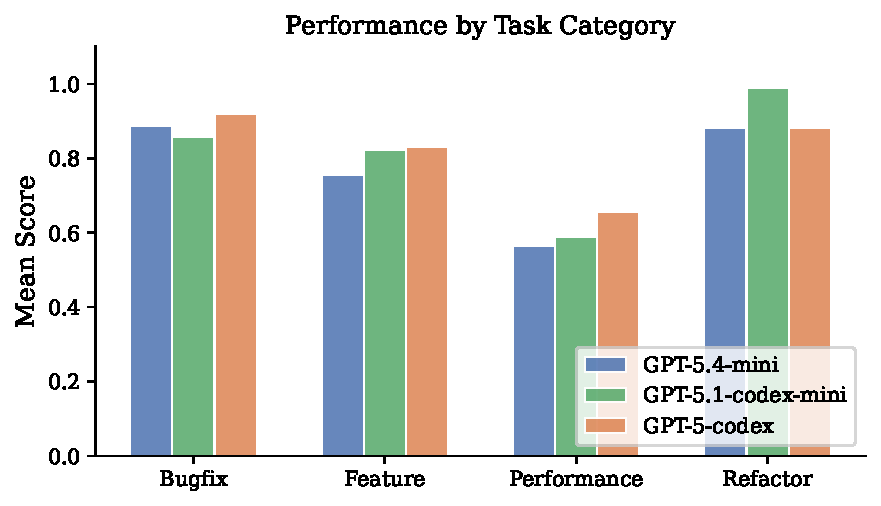
\includegraphics[width=0.85\textwidth]{figures/category_scores.pdf}
\caption{Mean score by task category for each model.}
\label{fig:categories}
\end{figure}

\subsection{Score Distribution}

Figure~\ref{fig:distribution} shows the score distribution across all three models. The distribution is strongly bimodal: tasks cluster either near 1.0 (fully solved) or below 0.5 (largely failed), with virtually no tasks falling in the [0.5, 0.7) range. This pattern holds across all three models and suggests that current agents exhibit a binary mode of engagement---they either correctly identify the required change and implement it to completion, or fail to make meaningful progress. Partial solutions, where an agent understands the problem direction but implements it incompletely, are surprisingly rare.

\begin{figure}[ht]
\centering
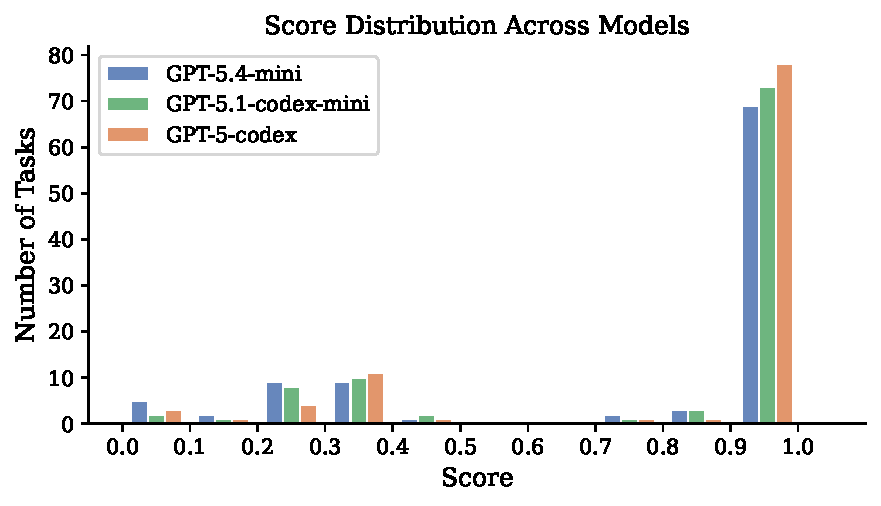
\includegraphics[width=0.85\textwidth]{figures/score_distribution.pdf}
\caption{Score distribution across all three models. The distribution is notably bimodal, with tasks clustering near 0.3 (no changes, only regression credit) and 1.0 (fully solved).}
\label{fig:distribution}
\end{figure}

\section{Shortcomings}

Several limitations of this benchmark merit discussion. The task mining process is biased toward recently updated pull requests, as the GitHub API sorts by update time. This overrepresents recent code patterns and undersamples older, potentially more fundamental algorithmic changes. The category imbalance---only 9 refactor and 11 performance tasks---limits the statistical power of per-category comparisons; confidence intervals on these subsets are wide.

The evaluation reflects the joint performance of the model and the mini-swe-agent scaffold, not the model's intrinsic coding capability in isolation. A different scaffold design---with different prompting strategies, tool availability, or exploration budgets---could alter the relative rankings. Additionally, all results are from single runs without pass@k analysis, so variance across attempts is unmeasured.

The scoring function is purely functional, evaluating only whether tests pass or fail. Two solutions that achieve identical test outcomes but differ substantially in readability, maintainability, or idiomatic style receive the same score. Finally, some PR descriptions in the dataset are underspecified, forcing agents to infer intent primarily from test names and failure messages rather than natural language requirements.

\section{Proposed Improvements}

Several directions would strengthen the benchmark. Scaling to 500 or more tasks by mining the full PR history and incorporating issue-linked pull requests would improve both diversity and statistical power. Running each task multiple times at temperature $> 0$ would enable pass@k analysis, distinguishing reliably solvable tasks from those that are only occasionally solved.

Auto-classifying tasks into difficulty tiers based on diff size, file count, and cyclomatic complexity would enable stratified analysis at the frontier of agent capability. Tracking efficiency metrics such as tokens consumed and wall-clock time per task would capture an important practical dimension: two models with equal scores but vastly different costs have very different deployment value.

Adding an LLM-as-judge component to evaluate code quality, readability, and adherence to project conventions would complement the functional score with a qualitative dimension. Extending the methodology to other pure-Python libraries such as scikit-image, Biopython, or librosa would test whether agent performance generalizes across codebases with different conventions and domain requirements. Finally, running identical models through multiple agent scaffolds---SWE-agent, Aider, OpenHands---would help disentangle model capability from scaffold design choices.

\section{Reproducibility}

All code, task definitions, and results are publicly available at \url{https://github.com/iskhare/nx-bench}. The evaluation can be reproduced with the following steps:

\begin{verbatim}
conda create -n nx-bench python=3.11 -y && conda activate nx-bench
git clone https://github.com/iskhare/nx-bench.git && cd nx-bench
git clone https://github.com/networkx/networkx.git
git clone https://github.com/SWE-agent/mini-swe-agent.git
cd mini-swe-agent && pip install -e . && cd ..
pip install -r requirements.txt
docker build -f Dockerfile.eval -t nx-eval .
python run_benchmark.py --output results/
python analyze.py results/
\end{verbatim}

\begin{thebibliography}{9}
\bibitem{swebench}
C.~E. Jimenez, J.~Yang, A.~Wettig, S.~Yao, K.~Pei, O.~Press, and K.~Narasimhan.
\newblock {SWE-bench}: Can Language Models Resolve Real-World {GitHub} Issues?
\newblock In \emph{Proceedings of ICLR}, 2024.
\newblock \url{https://github.com/princeton-nlp/SWE-bench}

\bibitem{networkx}
A.~A. Hagberg, D.~A. Schult, and P.~J. Swart.
\newblock Exploring network structure, dynamics, and function using {NetworkX}.
\newblock In \emph{Proceedings of the 7th Python in Science Conference (SciPy)}, pages 11--15, 2008.
\newblock \url{https://github.com/networkx/networkx}

\bibitem{minisweagent}
J.~Yang, C.~E. Jimenez, K.~Narasimhan, and O.~Press.
\newblock mini-swe-agent: A lightweight agent scaffold for software engineering tasks.
\newblock 2024.
\newblock \url{https://github.com/SWE-agent/mini-swe-agent}
\end{thebibliography}

\end{document}
